\documentclass[landscape,final,a0paper]{baposter}


\tracingstats=2

\usepackage{calc}
\usepackage{graphicx}
\usepackage{amsmath}
\usepackage{amssymb}
\usepackage{relsize}
\usepackage{multirow}
\usepackage{bm}

\usepackage{graphicx}
\usepackage{multicol}

\usepackage{pgfbaselayers}
\pgfdeclarelayer{background}
\pgfdeclarelayer{foreground}
\pgfsetlayers{background,main,foreground}

\usepackage{times}
\usepackage{helvet}
\usepackage{palatino}

\newcommand{\captionfont}{\footnotesize}

\selectcolormodel{cmyk}

%\graphicspath{{images/}}

%%%%%%%%%%%%%%%%%%%%%%%%%%%%%%%%%%%%%%%%%%%%%%%%%%%%%%%%%%%%%%%%%%%%%%%%%%%%%%%%
%%%% Some math symbols used in the text
%%%%%%%%%%%%%%%%%%%%%%%%%%%%%%%%%%%%%%%%%%%%%%%%%%%%%%%%%%%%%%%%%%%%%%%%%%%%%%%%
% Format 

\renewcommand{\Pr}{\mbox{P}}
\newcommand{\e}{\mbox{e}}
\newcommand{\dx}{\,\mbox{d}x}

%%%%%%%%%%%%%%%%%%%%%%%%%%%%%%%%%%%%%%%%%%%%%%%%%%%%%%%%%%%%%%%%%%%%%%%%%%%%%%%%
% Multicol Settings
%%%%%%%%%%%%%%%%%%%%%%%%%%%%%%%%%%%%%%%%%%%%%%%%%%%%%%%%%%%%%%%%%%%%%%%%%%%%%%%%
\setlength{\columnsep}{0.7em}
\setlength{\columnseprule}{0mm}


%%%%%%%%%%%%%%%%%%%%%%%%%%%%%%%%%%%%%%%%%%%%%%%%%%%%%%%%%%%%%%%%%%%%%%%%%%%%%%%%
% Save space in lists. Use this after the opening of the list
%%%%%%%%%%%%%%%%%%%%%%%%%%%%%%%%%%%%%%%%%%%%%%%%%%%%%%%%%%%%%%%%%%%%%%%%%%%%%%%%
\newcommand{\compresslist}{%
\setlength{\itemsep}{1pt}%
\setlength{\parskip}{0pt}%
\setlength{\parsep}{0pt}%
}


%%%%%%%%%%%%%%%%%%%%%%%%%%%%%%%%%%%%%%%%%%%%%%%%%%%%%%%%%%%%%%%%%%%%%%%%%%%%%%
%%% Begin of Document
%%%%%%%%%%%%%%%%%%%%%%%%%%%%%%%%%%%%%%%%%%%%%%%%%%%%%%%%%%%%%%%%%%%%%%%%%%%%%%

\begin{document}

%%%%%%%%%%%%%%%%%%%%%%%%%%%%%%%%%%%%%%%%%%%%%%%%%%%%%%%%%%%%%%%%%%%%%%%%%%%%%%
%%% Here starts the poster
%%%---------------------------------------------------------------------------
%%% Format it to your taste with the options
%%%%%%%%%%%%%%%%%%%%%%%%%%%%%%%%%%%%%%%%%%%%%%%%%%%%%%%%%%%%%%%%%%%%%%%%%%%%%%
% Define some colors
\definecolor{silver}{cmyk}{0,0,0,0.3}
\definecolor{yellow}{cmyk}{0,0,0.9,0.0}
\definecolor{reddishyellow}{cmyk}{0,0.22,1.0,0.0}
\definecolor{black}{cmyk}{0,0,0.0,1.0}
\definecolor{darkYellow}{cmyk}{0,0,1.0,0.5}
\definecolor{darkSilver}{cmyk}{0,0,0,0.1}
\definecolor{lightyellow}{cmyk}{0,0,0.3,0.0}
\definecolor{lighteryellow}{cmyk}{0,0,0.1,0.0}
\definecolor{lighteryellow}{cmyk}{0,0,0.1,0.0}
\definecolor{lightestyellow}{cmyk}{0,0,0.05,0.0}
\definecolor{cyan}{cmyk}{1,0,0,0}
\definecolor{lightcyan}{cmyk}{0.5,0,0,0}
\definecolor{pastelcyan}{cmyk}{0.25,0,0,0}
\definecolor{magenta}{cmyk}{0,1,0,0}
\definecolor{yellow}{cmyk}{0,0,1,0}
\definecolor{lightyellow}{cmyk}{0,0,0.5,0}
\definecolor{pastelyellow}{cmyk}{0,0,0.25,0}
\definecolor{black}{cmyk}{0,0,0,1}
\definecolor{darkgray}{cmyk}{0,0,0,0.75}
\definecolor{gray}{cmyk}{0,0,0,0.5}
\definecolor{lightgray}{cmyk}{0,0,0,0.25}
\definecolor{white}{cmyk}{0,0,0,0}
\definecolor{red}{cmyk}{0,1,1,0}
\definecolor{orange}{cmyk}{0,0.5,1,0}
\definecolor{scarlet}{cmyk}{0,1,0.5,0}
\definecolor{brown}{cmyk}{0.5,0.75,1,0}
\definecolor{camel}{cmyk}{0.25,0.375,0.5,0}
\definecolor{cream}{cmyk}{0,0.2,0.3,0}
\definecolor{green}{cmyk}{1,0,1,0}
\definecolor{lightgreen}{cmyk}{0.5,0,0.5,0}
\definecolor{pastelgreen}{cmyk}{0.25,0,0.25,0}
\definecolor{mossgreen}{cmyk}{0.64,0.4,1,0}
\definecolor{yellowgreen}{cmyk}{0.5,0,1,0}
\definecolor{skyblue}{cmyk}{0.4,0.16,0,0}
\definecolor{royal}{cmyk}{1.0,0.5,0,0}
\definecolor{navyblue}{cmyk}{0.9,0.75,0.5,0}
\definecolor{lightnavy}{cmyk}{0.4,0.3,0.2,0}
\definecolor{blue}{cmyk}{1,1,0,0}
\definecolor{lightblue}{cmyk}{0.5,0.5,0,0}
\definecolor{pastelblue}{cmyk}{0.25,0.25,0,0}
\definecolor{lightpastelblue}{cmyk}{0.15,0.15,0,0}
\definecolor{lightestpastelblue}{cmyk}{0.05,0.05,0,0}
\definecolor{lavender}{cmyk}{0.25,0.25,0,0}
\definecolor{violet}{cmyk}{0.75,1,0.25,0}
\definecolor{purple}{cmyk}{0.5,1,0.5,0}
\definecolor{lightpurple}{cmyk}{0.25,0.5,0.25,0}
\definecolor{pink}{cmyk}{0,0.5,0,0}


%%

\typeout{Poster Starts}
%\background{
  %\begin{tikzpicture}[remember picture,overlay]%
  %  \draw (current page.north west)+(-2em,-2em) node[anchor=north west] %{\hspace{-2em}\includegraphics[height=1.1\textheight]{silhouettes_background}};
 % \end{tikzpicture}%
%}




\newlength{\leftimgwidth}
\begin{poster}%
  % Poster Options, such as colours etc
  {
  % Show grid to help with alignment
  grid=false,
 % Column spacing
  colspacing=0.5em,
 % Color style
 % bgColorOne=pastelblue,
 %bgColorTwo=lightpastelblue,
  bgColorOne=white,
  bgColorTwo=white,
  borderColor=navyblue,
  headerColorOne=lightnavy,
  headerColorTwo=purple,
  headerFontColor=black,
 % boxColorOne=lightpastelblue,
 % boxColorTwo=lightestpastelblue,
 boxColorOne=white,
 boxColorTwo=white,
 % Format of textbox
  textborder=roundedleft,
% textborder=rectangle,
% Format of text header
  eyecatcher=true,
  headerborder=open,
  headerheight=0.08\textheight,
  headershape=roundedright,
  headershade=plain,
  headerfont=\Large\textsf, %Sans Serif
  boxshade=plain,
%  background=shade-tb,
 % background=plain,
  background=none,
  linewidth=2pt
  }
  % Eye Catcher
  {
\includegraphics[width=10em]{correlation.png}} % select eyecatcher=false above if not required. If no eye catcher is present, the title is left aligned.
  % Title
  {\sf %Sans Serif
  %\bf% Serif
  Random bits of M1S}
  % Authors
  {\sf %Sans Serif
  % Serif
  \vspace{1em} 
	Emma McCoy
  }
  % University logo
  { % The makebox allows the title to flow into the logo
    \makebox[8em][r]{%
        \begin{minipage}{16em}
				\hfill 
\includegraphics[height=3em]{imperial.pdf}
				\end{minipage}
      
    }
  }

  \tikzstyle{light shaded}=[top color=baposterBGtwo!30!white,bottom color=baposterBGone!30!white,shading=axis,shading angle=30]

  % Width of left inset image
     \setlength{\leftimgwidth}{0.78em+8.0em}

%%%%%%%%%%%%%%%%%%%%%%%%%%%%%%%%%%%%%%%%%%%%%%%%%%%%%%%%%%%%%%%%%%%%%%%%%%%%%%
%%% Now define the boxes that make up the poster
%%%---------------------------------------------------------------------------
%%% Each box has a name and can be placed absolutely or relatively.
%%% The only inconvenience is that you can only specify a relative position 
%%% towards an already declared box. So if you have a box attached to the 
%%% bottom, one to the top and a third one which should be in between, you 
%%% have to specify the top and bottom boxes before you specify the middle 
%%% box.
%%%%%%%%%%%%%%%%%%%%%%%%%%%%%%%%%%%%%%%%%%%%%%%%%%%%%%%%%%%%%%%%%%%%%%%%%%%%%%
    %
    % A coloured circle useful as a bullet with an adjustably strong filling
\newcommand{\colouredcircle}[1]{%
      \tikz{\useasboundingbox (-0.2em,-0.32em) rectangle(0.2em,0.32em); \draw[draw=black,fill=baposterBGone!80!black!#1!white,line width=0.03em] (0,0) circle(0.18em);}}

%%%%%%%%%%%%%%%%%%%%%%%%%%%%%%%%%%%%%%%%%%%%%%%%%%%%%%%%%%%%%%%%%%%%%%%%%%%%%%
  \headerbox{Outline}{name=outline,column=0,row=0}{
%%%%%%%%%%%%%%%%%%%%%%%%%%%%%%%%%%%%%%%%%%%%%%%%%%%%%%%%%%%%%%%%%%%%%%%%%%%%%%
``Lies, damn lies and statistics."
-- Mark Twain. \\
Luckily, this course is about probability, so I can leave the lies to the second year lecturers....

Assessment of uncertainty in such real-life problems is a complex
issue which requires a rigorous mathematical treatment.
M1S develops the probability framework in which
questions of practical interest can be posed and resolved.
	\vspace{0.3em}
 }

%%%%%%%%%%%%%%%%%%%%%%%%%%%%%%%%%%%%%%%%%%%%%%%%%%%%%%%%%%%%%%%%%%%%%%%%%%%%%%
  \headerbox{Contents}{name=contents,column=0,below=outline}{
%%%%%%%%%%%%%%%%%%%%%%%%%%%%%%%%%%%%%%%%%%%%%%%%%%%%%%%%%%%%%%%%%%%%%%%%%%%%%%
    The course will cover the following topics
		\begin{enumerate}
\item SAMPLE SPACES AND EVENTS
\item PROBABILITY: DEFINITIONS, INTERPRETATIONS
\item CONDITIONAL\ PROBABILITY
\item COMBINATORICS
\item DISCRETE\ RANDOM\ VARIABLES\ 
\item  CONTINUOUS\ RANDOM\ VARIABLES
\item  TRANSFORMATIONS
\item JOINT DISTRIBUTIONS
\end{enumerate}
I will cut and paste various bits of \LaTeX  from the coursenotes and some plots from my MSc course in nonparametric regressions to produce this poster.
  \vspace{0.3em}
  }

%%%%%%%%%%%%%%%%%%%%%%%%%%%%%%%%%%%%%%%%%%%%%%%%%%%%%%%%%%%%%%%%%%%%%%%%%%%%%%
  \headerbox{Sample Space and Events}{name=sample,column=0,below=contents}{
%%%%%%%%%%%%%%%%%%%%%%%%%%%%%%%%%%%%%%%%%%%%%%%%%%%%%%%%%%%%%%%%%%%%%%%%%%%%%%
   The set of {\bf all} possible outcomes is called the {\bf SAMPLE SPACE}, $\Omega$.
\\ \\
If $\omega$ is a possible outcome, $\omega \in \Omega$.
\[
\Omega = \{\omega_1, \omega_2, \ldots\}
\]
$\omega_1, \omega_2, \ldots$ are {\bf elements} of $\Omega$.
\\ \\
Subsets of $\Omega$ are called {\bf EVENTS}.\\
{\bf DE MORGAN'S LAWS}
\begin{enumerate}
\item $(E \cup F)' = E' \cap F'$.
\item $(E \cap F)' = E' \cup F'$.
\end{enumerate}
This can be extended to countably infinite events.
  \vspace{0.3em}
  }

%%%%%%%%%%%%%%%%%%%%%%%%%%%%%%%%%%%%%%%%%%%%%%%%%%%%%%%%%%%%%%%%%%%%%%%%%%%%%%
 

%%%%%%%%%%%%%%%%%%%%%%%%%%%%%%%%%%%%%%%%%%%%%%%%%%%%%%%%%%%%%%%%%%%%%%%%%%%%%%
  \headerbox{Combinatorics}{name=comb,column=1,span=2, row=0}{
	{\bf Definition}
\\
An {\bf ordered} arrangement of $r$ items from $n$ is a {\bf PERMUTATION}.
\\The number of ordered sample of $r$ items from a population
of size $n$ ( $r \leq n$) is
\begin{align*}
^n P_r &= \frac{n!}{(n-r)!} = (n)_r \\
&= n(n-1) \ldots (n-r+1).
\end{align*}
{\bf Definition}
\\
An {\bf unordered} arrangement of $r$ items from $n$ is a {\bf COMBINATION}.
\\The number of unordered samples of size $r$ items from a population
of size $n$ ( $r \leq n$) is
\begin{align*}
^n C_r &= \frac{n!}{r!(n-r)!} = {n \choose r}.
\end{align*}
{\bf SUMMARY} \\ 
total number of samples of $r$ from $n$:
\\
\begin{tabular}{lcc}
& \multicolumn{1}{c}{WITHOUT} & \multicolumn{1}{c}{WITH} \\
& \multicolumn{1}{c}{REPLACEMENT} & \multicolumn{1}{c}{REPLACEMENT}\\
ORDERED & $(n)_r$ & $n^r$ \\
UNORDERED & ${n \choose r}$ & ${n+r-1 \choose r}$\\
\end{tabular}	

 }


%%%%%%%%%%%%%%%%%%%%%%%%%%%%%%%%%%%%%%%%%%%%%%%%%%%%%%%%%%%%%%%%%%%%%%%%%%%%%%
\headerbox{Some Graphics}{name=plots,column=1,span=2,below=comb}{

\begin{minipage}[c]{8cm}
Here are some random plots:\\
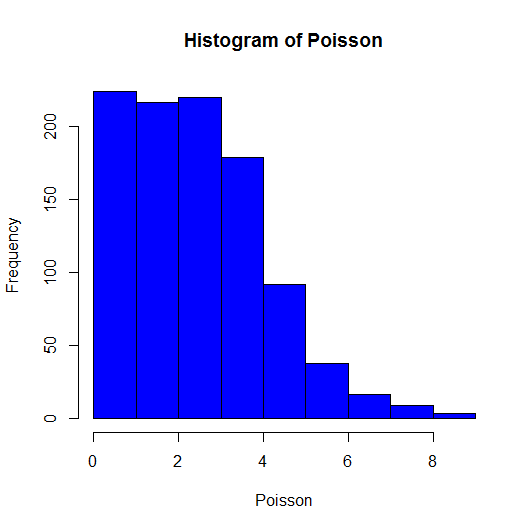
\includegraphics[width=2.5cm]{poisson.png}
  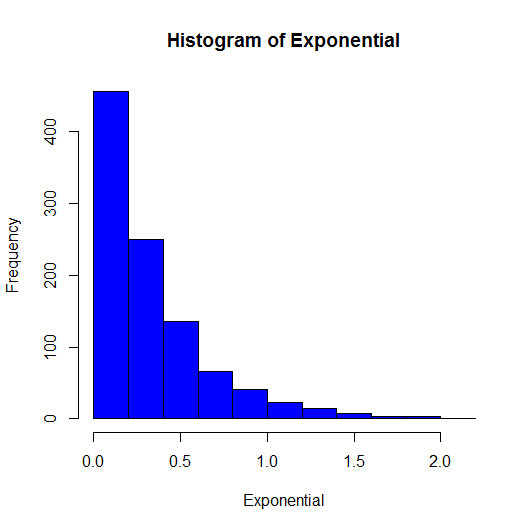
\includegraphics[width=2.5cm]{exp.png}
    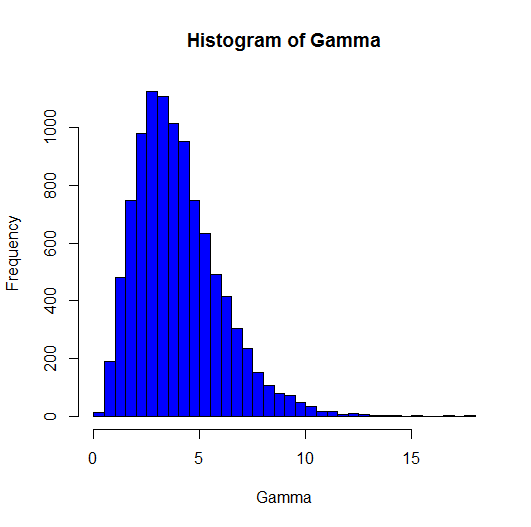
\includegraphics[width=2.5cm]{gamma.png}

   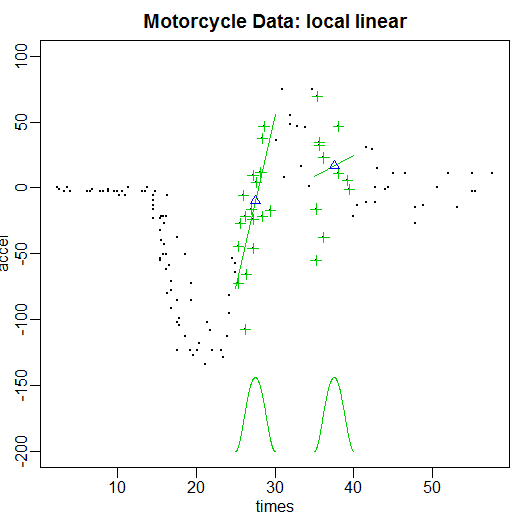
\includegraphics[width=2.5cm]{mcycle.png}
    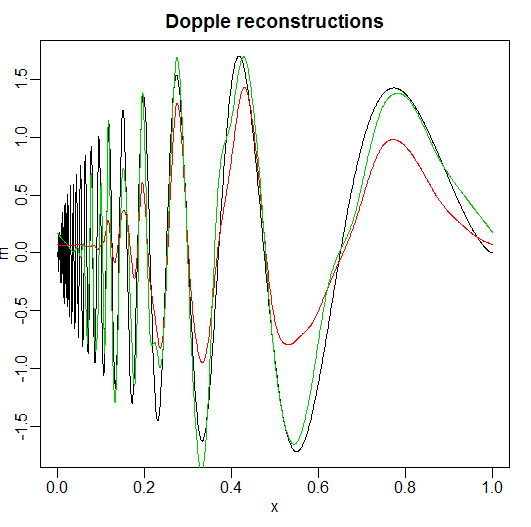
\includegraphics[width=2.5cm]{doppler.png}
   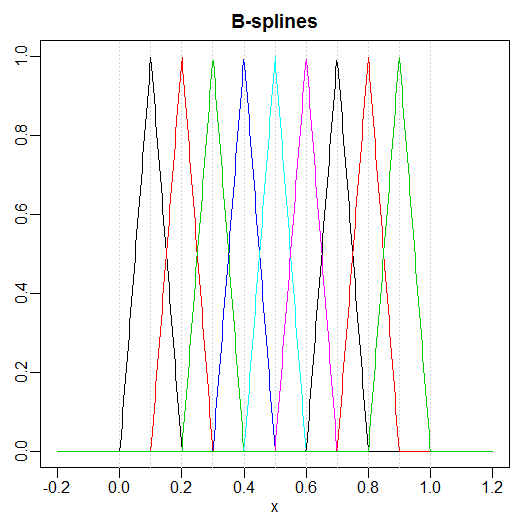
\includegraphics[width=2.5cm]{bsplines.png}
\end{minipage}
\begin{minipage}[c]{8cm}
here is some random text, which is in a minipage which allows you to add complicated stuff, e.g. lists and more maths:
\begin{enumerate}
\item histograms for three distribitions:
\begin{enumerate}
\item Poisson
\item Exponential
\item Gamma
\end{enumerate}
\item Plots taken from the non-parametric regression MSc course
\end{enumerate}
\end{minipage}
	
  \vspace{0.5em}
  }

%%%%%%%%%%%%%%%%%%%%%%%%%%%%%%%%%%%%%%%%%%%%%%%%%%%%%%%%%%%%%%%%%%%%%%%%%%%%%%
  \headerbox{Discrete Random Variables}{name=discrete,column=3,row=0}{
  Bernoulli distribution:   
	\begin{align*}
f_X(x)& = \left\{ \begin{array}{ll}
1-\theta \qquad & x=0; \\
\theta & x=1, 
\end{array}\right. \\
&= \theta^x (1-\theta)^{1-x} \quad x \in \{0,1\},
\end{align*}
 for $0 \leq \theta \leq 1$.  \\

	Binomial distribution
	\[
f_X(x) = \Pr(X=x) = {n \choose x} \theta^x (1-\theta)^{n-x},
\]
for $0 \leq x \leq n$, and zero otherwise.\\
  \vspace{0.2em}
  }


%%%%%%%%%%%%%%%%%%%%%%%%%%%%%%%%%%%%%%%%%%%%%%%%%%%%%%%%%%%%%%%%%%%%%%%%%%%%%%
 \headerbox{Continuous Random Variables}{name=continuous,column=3,below=discrete}{
  Exponential Distribution
	\[
f_X(x) = \lambda \e^{-\lambda x} \quad x>0,
\]
for $\lambda >0$.\\ \\
Gamma Disbribution: 
\[
f_Y(y) = \frac{\beta^\alpha}{\Gamma(\alpha)} y^{\alpha-1} e^{-\beta y} \quad y>0,
\]
\begin{tabbing}
where \= $\alpha=$ shape \\
\> $\beta=$ scale
\end{tabbing}
Standard normal distribution:
\[
f_X(x) = \sqrt{\frac{1}{2\pi}} \exp\left(-\frac{1}{2} x^2\right).
\]
  \vspace{0.2em}
  }




%%%%%%%%%%%%%%%%%%%%%%%%%%%%%%%%%%%%%%%%%%%%%%%%%%%%%%%%%%%%%%%%%%%%%%%%%%%%%
\headerbox{Axioms of Probability}{name=axioms,column=1,below=plots}{
   {\bf Axioms of Probability} \\
For events $E, F \subseteq \Omega$ 
\begin{tabbing}
\hspace{.5cm} \= {\bf (I)} \hspace{.5cm} \=  $0 \leq \Pr(E) \leq 1$, \\
\> {\bf (II)} \> $\Pr(\Omega) = 1$,\\
\> {\bf (III)} \>  If $E \cap F = \phi$, then \\
\> \> $\Pr(E \cup F) = \Pr(E)+\Pr(F)$,\\
\> \>(Addition rule).
\end{tabbing}
  \vspace{0.3em}
  }

%%%%%%%%%%%%%%%%%%%%%%%%%%%%%%%%%%%%%%%%%%%%%%%%%%%%%%%%%%%%%%%%%%%%%%%%%%%%%
\headerbox{Conditional Probability}{name=cond,column=2,below=plots}{
For events $E, F \subseteq \Omega$, the conditional probability of $E$ given $F$ is defined as,
\[
\Pr(E \mid F) = \frac{\Pr( E \cap F)}{\Pr(F)}
\]
From which we can derive Bayes theorem:
\[
\Pr(E \mid F) = \frac{\Pr( F \cap E)\Pr(E)}{\Pr(F)}
\]
  }

%%%%%%%%%%%%%%%%%%%%%%%%%%%%%%%%%%%%%%%%%%%%%%%%%%%%%%%%%%%%%%%%%%%%%%%%%%%%%%
\headerbox{Conclusions}{name=concl,column=3,below=continuous}{
	Pretty easy to put boxes exactly where you like! just use the below and above commands.  Use the span command to span multiple columns. 
	}
	
%%%%%%%%%%%%%%%%%%%%%%%%%%%%%%%%%%%%%%%%%%%%%%%%%%%%%%%%%%%%%%%%%%%%%%%%%%%%%%
  \headerbox{References}{name=references,column=3,above=bottom}{
    \smaller
    \vspace{-0.4em}
    \bibliographystyle{plain}
    \renewcommand{\section}[2]{\vskip 0.05em}
      \begin{thebibliography}{1}\itemsep=-0.01em
      \setlength{\baselineskip}{0.4em}
      \bibitem{stir}
        D. Stirzaker.
        \newblock Elementary Probability. 
        \newblock Cambridge University Press, 2003.
      \bibitem{ross}
        S. Ross.
        \newblock A First Course in Probability.
        \newblock Prentice Hall, 2001.
				\bibitem{grimmett}
				G. Grimmett. 
				\newblock Probability and Random Processes.
				\newblock Oxford University Press, 2001.
      \end{thebibliography}
  }
%%%%%%%%%%%%%%%%%%%%%%%%%%%%%%%%%%%%%%%%%%%%%%%%%%%%%%%%%%%%%%%%%%%%%%%%%%%%%%
  
\end{poster}

\end{document}
